\chapter{Materials \& Methods}

For this \ac{IAPT} a multi-stage approach was used for data collection, analyses and evaluation.
This approach is described in figure~\ref{fig:flowchart} as a flowchart.

\begin{figure}[h!]
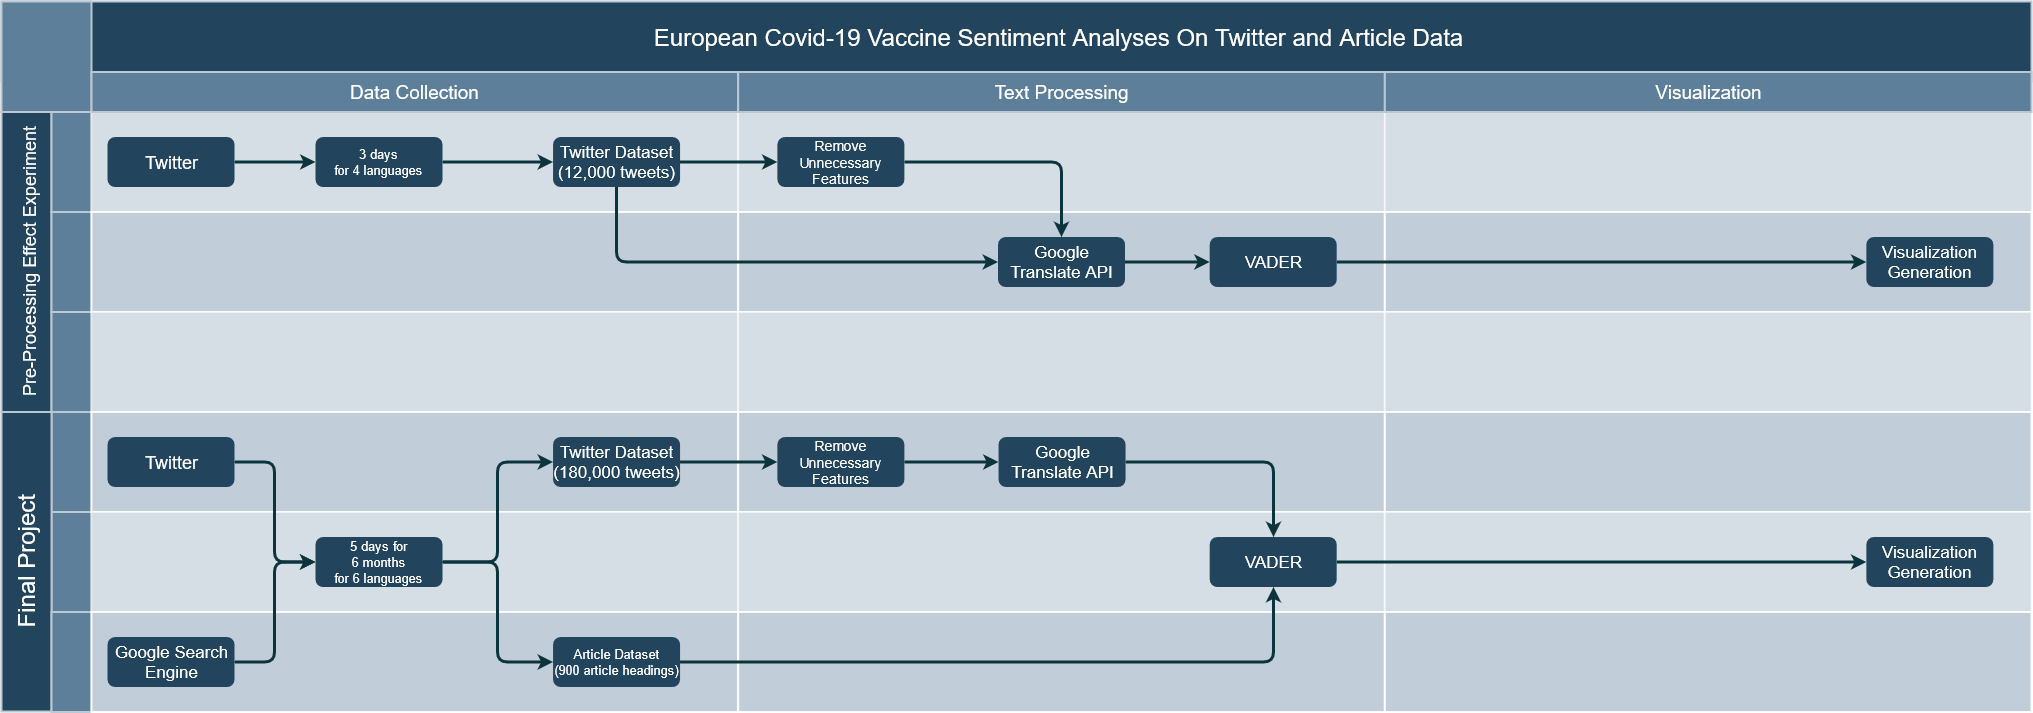
\includegraphics[scale=0.2]{IAPT Flowchart}
\caption[Method Flowchart]{Flowchart of the Method of Experiment\index{Method Flowchart}}
\label{fig:flowchart}
\end{figure}

\section{Data Collection}

\subsection{Twitter Dataset}

The large scale dataset of tweets maintained by \citet{banda2020largescale} is very large and analysing it in its entirety would be expensive, lengthy and out of scope for this \ac{IAPT}, since the majority of the data present is generated outside of the \ac{EU} borders.
The dataset contains daily folders representing each each day from the 22nd of March 2020, which contain two files, one of all tweets and retweets on the day, and the other a cleaned version with no retweets.
Instead all of this available data for every month from December 2020 till May 2021, 5 dates, the 1st, 7th, 14th, 21st, 28th where chosen and the clean dataset file was used.
It was decided that 1000 tweets from 6 languages would suffice to form the Twitter dataset.
The 6 languages, English, Spanish, French, German, Italian and Dutch are the European languages with the most presence in the Panacea Lab dataset.
An important point to consider when using the Panacea Lab dataset is that only the tweet ID is available.
However this ID can be easily used to download and collect the tweet text and other tweet features.
For this \ac{IAPT} the Python library, Tweepy a Python wrapper for the Twitter \ac{API} was used ~\citep{roesslein2020tweepy}.
The use of the Twitter \ac{API} requires the signing-up to the service with Twitter, where after approval \ac{API} are shared.
The free version comes with limitations such as a limit of 300 lookups/ 15 minutes, however a limit on status retrieval through the ID does not exist.
Hence for this part of the data collection no limitations were imposed by the Twitter \ac{API}.
In total 180,000 tweets where collected.

A smaller dataset was also collected following the same method as described above.
This smaller dataset features a 1000 tweets from 3 dates, the 1st of January, February and March and 4 languages, English, Spanish, French, German.
This dataset was used to test the effect of pre-processing the tweets before passing them to a \ac{VADER} model.
In total 12,000 tweets where collected.

\subsection{Article Dataset}

As the focus of this \ac{API} was explained to be more directed towards using social media data, it was decided that the article dataset would be much smaller in scale.
Using the Google search engine a query was done for every day a file was taken from the Panacea Lab dataset.
The query was of the format: \\\textquote{{Country} Covid* before:{Date in YYYY-MM-DD Format} After:{Day before Date in YYYY-MM-DD Format}}\\
5 relevant articles where collected for each day and stored in a number of csv files.
In total 900 articles where collected.

\section{Data Processing}

The tweet data collected is unfiltered and contain a number of useless features such as links, stop words and whitespace.
In the first part of this \ac{IAPT} the results of pre-processed tweets and 'naked' tweets are used to create a final pre-process function.
In the final version tweets go through the following process:

\begin{itemize}
    \item HTML special entities (e.g.\ \&amp;) are removed.
    \item Tickers are removed.
    \item Hyperlinks are removed.
    \item Punctuation is removed.
    \item "'s", "'t", "'ve" are split with a space.
    \item Words with 2 or fewer letters are removed.
    \item Whitespace is removed.
    \item Stop words are removed.
\end{itemize}

\noindent The stop word list for the various languages where taken from the \ac{NLTK} ~\citep{bird2009natural} library.
Article headings in the article dataset do not go through this pre-processing step.

For translation, non-English pre-processed tweet text was passed sent to the Google Cloud Translation \ac{API}.
The total cost of using the translation \ac{API} came to €60.
Article headings where not translated as they where collected only in English.

\section{Sentiment Analyses}

The \ac{NLTK} ~\citep{bird2009natural} library was employed to implement a \ac{VADER} ~\citep{Hutto_Gilbert_2014} model.
Each tweet and article heading was used as an input and the compound \ac{SA} score was kept.
The mean compound score of each day was stored in a file, while each score was classifies as either:

\begin{itemize}
    \item very positive (score >= 0.75)
    \item positive (0.25 <= score < 0.75)
    \item neutral (-0.25 <= score < 0.25)
    \item negative (-0.75 <= score < 0.25)
    \item very negative (score < -0.75)
\end{itemize}

\section{Visualization}

The \ca{SA} scores where visualized via the use of Time Series plots and word clouds for each month.
The focus of these visualizations was aimed at the results stemming from the Twitter dataset.
Discussion on the visualizations produced are found in the following chapter, Results \& Discussion.